\documentclass[a4paper,12pt]{report}
 
% Différentes options pour la classe :
% - taille de la fonte    : 10pt, 11pt, 12pt
% - recto ou recto-verso    : oneside, twoside
% - stade de développement    : draft, final
 
% Chargement d'extensions
\usepackage[latin1,utf8]{inputenc}    % Pour utiliser les lettres accentuées
\usepackage[francais]{babel}    % Pour la langue française
\usepackage{graphicx}
 
% Informations le titre, le(s) auteur(s), la date
\title{Rapport de projet : Etrange}
\author {Caroline Keramsi, Florian Thorey, Samuel Mokrani}
\date{\today}
 
% Début du document
\begin{document}
 
\maketitle
\tableofcontents    % Table des matières
\listoffigures        % Liste des figures
 
    \chapter*{Introduction}
    \addcontentsline{toc}{chapter}{Introduction}
{Dans le cadre du cours de System On Chips à Télécom Paristech, nous avons du réaliser
un module de traitement vidéo. Plus précisément, ce module doit être capable à partir d'un flux vidéo d'entrée représentée en 256 niveaux de gris, d'établir une transformation géométrique d'ordre 3. Voici les images que nous pouvons obtenir suite à une telle transformation :}
 
\begin{figure}[!h]
	\centering
	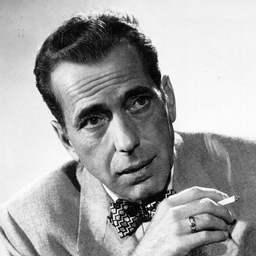
\includegraphics[scale = 0.5]{bogart.png}
	\caption{Image non transformée}
\end{figure}

\begin{figure}[!h]
	\centering
	
\includegraphics[scale = 0.5]{bogart_tr.png}
	\caption{Image transformée}
\end{figure}

{///////TODO : explication de l'algo backward machin}

	\part{Architecture retenue}
	\section*{Architecture retenue}
	\addcontentsline{toc}{section}{Architecture retenue}
{Pour réaliser ce module de traîtement vidéo, nous avons décidé d'utiliser l'architecture suivante :
 
\begin{figure}[!h]
	\centering
	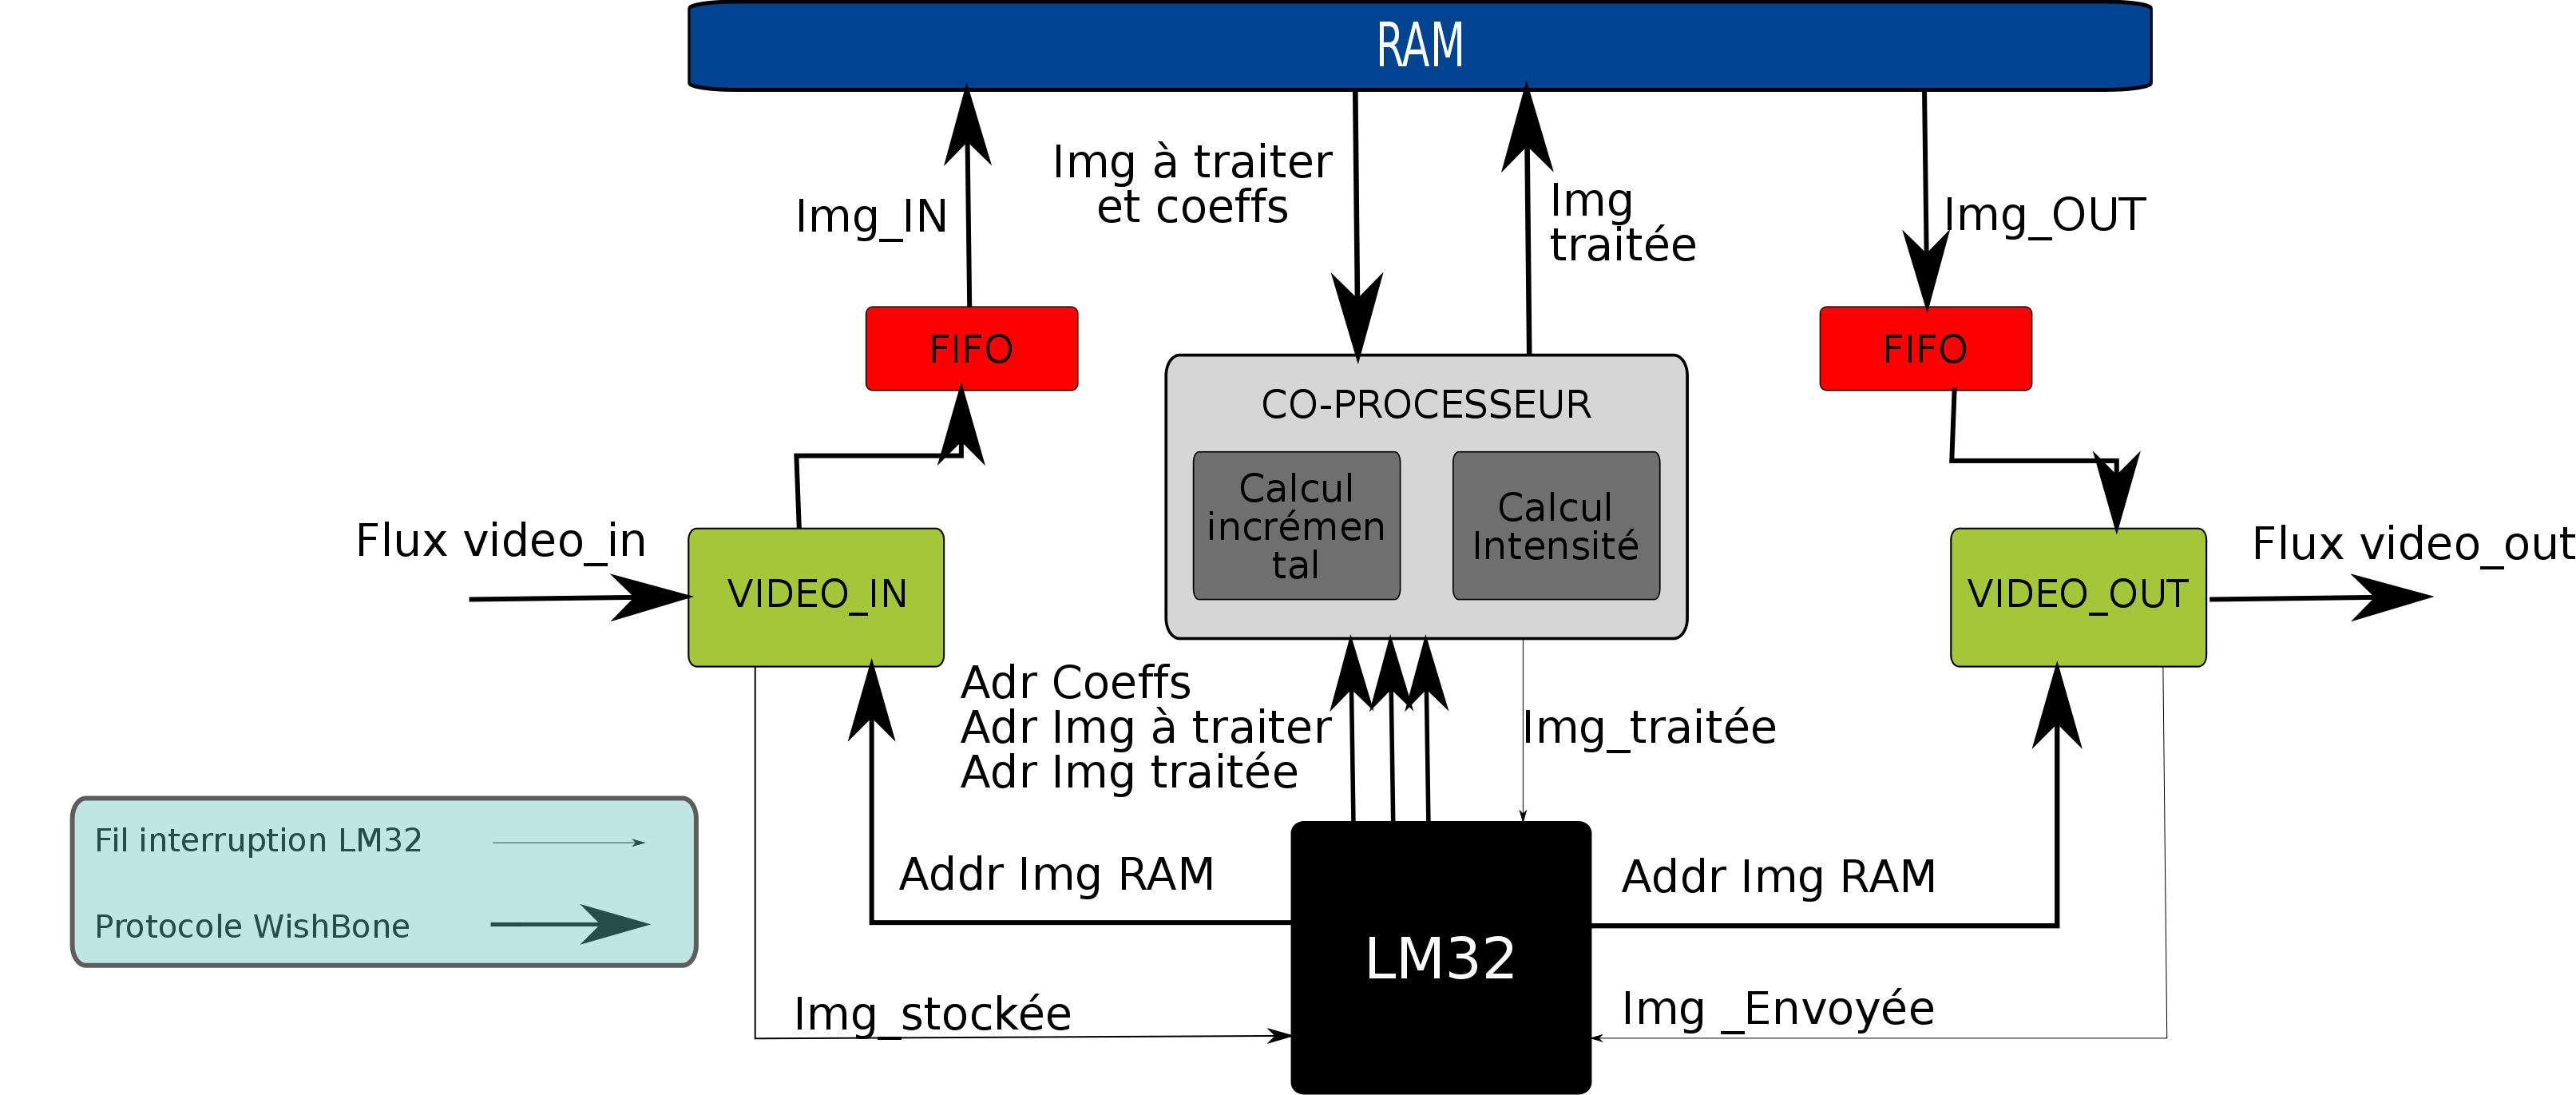
\includegraphics[scale = 0.1]{hardware-arch.png}
	\caption{Architecture}
\end{figure}

Le module VidéoIn se charge de mettre le flux entrant en RAM. VidéoCalc se charge d'aller lire en RAM une image à traîter et à mettre à un autre endroit de la RAM l'image traîtée. Enfin, le module VidéoOut se charge d'aller lire l'image traîtée et de générer un nouveau flux vidéo. Tous ces modules seront pilotés par le processeur (LM32) par le biais d'interruptions. Il enverra aux différents modules les bonnes adresses pour aller lire et écrire en RAM.


Cette architecture a l'avantage d'être modulaire. Par exemple, on peut ne pas utiliser le module de transformation juste en changeant le programme tournant sur le processeur.
}






    \part{VidéoIn / VidéoOut}

    \section*{VidéoIn}
    \addcontentsline{toc}{section}{VidéoIn}

{}

\newpage
 
    \section*{VidéoOut}
    \addcontentsline{toc}{section}{VidéoOut}

{}
     








    \part{VidéoCalc} 
    \section*{VidéoCalc}
    \addcontentsline{toc}{section}{VidéoCalc}

{}










    \part{Soft (LM32)} 

    \section*{Soft (LM32)}
    \addcontentsline{toc}{section}{Soft (LM32)}

{Le processeur a la charge d'indiquer aux différents modules les adresses à aller lire et écrire les images. Plus précisément :

\begin{itemize}
	\item VidéoIn : envoie de l'adresse où l'image entrante sera stockée
	\item VidéoCalc : \begin{itemize}
								\item envoie de l'adresse où sera lue l'image à traitée
								\item envoie de l'adresse où sera stockée l'image traîtée
								\item envoie de l'adresse du début des coefficients pour le calcul incrémental
							\end{itemize}
	\item VidéoOut : envoie de l'adresse où sera lue l'image traîtée
\end{itemize}

Toutes ces adresses sont envoyées suites à des interruptions.
}



 
    \chapter*{Conclusion}
    \addcontentsline{toc}{chapter}{Conclusion}
{}


% Fin du document
\end{document}
